\subsection{Dreiecksformeln}
\begin{tabular}{lll}
	& \parbox{9.5cm}{
		\textbf{Cosinussatz} \\
		$$c^2 = a^2 + b^2 - 2 \cdot a \cdot b \cdot \cos \gamma$$\\
		\textbf{Sinussatz} \\
		$$\frac{a}{\sin \alpha} = \frac{b}{\sin \beta} = \frac{c}{\sin \gamma} = 2r =
		\frac{u}{\pi}$$
		\textbf{Pythagoras beim Sinus}\\
		$$\sin^2(b)+\cos^2(b)=1 \qquad \tan(b)=\frac{\sin(b)}{\cos(b)}$$}
		
	& \parbox{8cm}{
		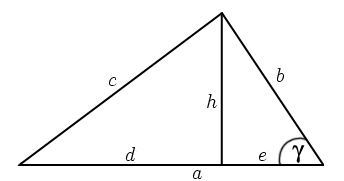
\includegraphics[width=6cm]{./idiotenseite/images/cosinussatz.png}}
\end{tabular}
\begin{center}
	\begin{multicols}{2}
		$\sin \beta = \frac ba =\frac{\text{Gegenkathete}}{\text{Hypotenuse}}$\\
		$\cos \beta = \frac ca =\frac{\text{Ankathete}}{\text{Hypotenuse}}$\\
		$\tan \beta = \frac cb =\frac{\text{Gegenkathete}}{\text{Ankathete}}$\\
		$\cot \beta = \frac cb =\frac{\text{Ankathete}}{\text{Gegenkathete}}$\\
	\end{multicols}
\end{center}

	